\section{Analysis of the Controller}\label{analysisController}
A first analysis of the controller can be done through the resultant Nyquist plot.

\begin{figure}[H] 
	\centering 
	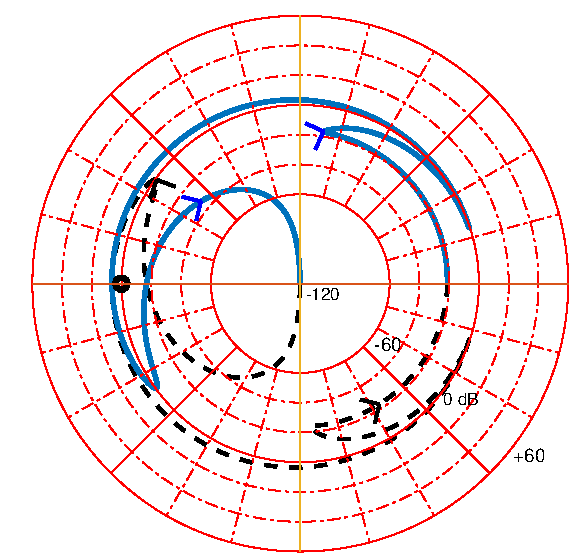
\includegraphics[scale=0.46]{figures/nyquistController}	
	\caption{Nyquist plot of the system with the controller}
	\label{nyquistController}
\end{figure}

Now the number of poles in the RHP is two and the number of encirclements around -1 is equals -2 (they are counterclockwise). This means that the system is stable, as the number of zeros in the RHP becomes 0.

Another step in the analysis is by means of a simulation, using the block diagram of the system.

The resultant system can be seen in figures XXX.

\fxnote{Include block diagram with the controller}

When a reference of 0 rad is given to the system, which has a tiny deviation from the equilibrium position in the initial condition, the behavior is the one shown in figures XXX and YYYYY. 

\fxnote{Include figure of the response}

As it can be seen, the controller is capable of balancing the Cubli at position 0 rad with a control action (torque) which can only take values from -0.134 to 0.134 as the real actuator does.